% advsync/rcu.tex

\section{Read-Copy Update}
\label{sec:advsync:Read-Copy Update}

Read-copy update (RCU) can be thought of as a replacement for
reader-writer locking for
which the read-side primitives are extremely light weight, and where
readers and writers do not exclude each other.
This last means that writers must leave old versions
of RCU-protected data structures
in place until all concurrent readers have completed,
so that RCU write-side primitives can be quite expensive.
RCU is thus best-suited for read-mostly situations, or for situations
in which realtime constraints require deterministic readers.

RCU provides the \url{rcu_read_lock()} and \url{rcu_read_unlock}
primitives to demark read-side critical sections, and
\url{synchronize_rcu} to allow writers to wait for completion
of all pre-existing readers.
The time that waiters much wait is termed a ``grace period''.
RCU read-side critical sections may be nested, which results in
the inner critical sections being subsumed into the outermost critical
section.

\subsection{RCU Read-Side Critical Sections and Grace Periods}
\label{sec:advsync:RCU Read-Side Critical Sections and Grace Periods}

Legal and illegal relationships of RCU read-side critical sections
to a grace periods are shown in
Figure~\ref{fig:advsync:RCU Readers and Grace Periods}.
Each blue box in the diagram represents an RCU read-side critical
section, as shown below.
The green box represents update-initiation code, for example, a
\url{list_del_rcu()} removing an element from an RCU-protected linked list,
with the color green representing the fact that readers can freely
access the element being removed.
The yellow box represents an RCU grace period, for example, a
\url{synchronize_rcu()}, with the color yell representing the fact that
pre-existing readers may still access the removed element, but new
readers cannot.
Finally, the red box represents completion
of the update, for example, a \url{kfree()} call to reclaim the removed
element's memory, with the color red indicating that no readers may
access the removed element.

\vspace{5pt}
\begin{minipage}[t]{\columnwidth}
\begin{verbatim}
rcu_read_lock();
/* RCU read-side critical section. */
rcu_read_unlock();
\end{verbatim}
\end{minipage}
\vspace{5pt}

\begin{figure}[htb]
\begin{center}
\resizebox{3in}{!}{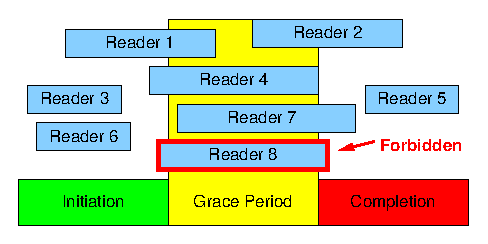
\includegraphics{advsync/RCUReaderGP}}
\end{center}
\caption{RCU Readers and Grace Periods}
\label{fig:advsync:RCU Readers and Grace Periods}
\end{figure}

This color coding indicates why it is forbidden for Reader~8 to
begin before the grace period starts, but persist until after the
grace period has ended.
This situation might permit Reader~8 to still be holding a reference
to the removed element, which could in turn result in memory corruption
failures.

So what happens if a reader executes for longer than planned?

The grace period extends in this case for as long as necessary to
accommodate any pre-existing reader, as shown in
Figure~\ref{fig:advsync:RCU Readers Extending Grace Periods}.
Note, however, that the grace period need not extend to cover Readers~2
and 8, since these two readers started after the beginning of the
grace period, and therefore cannot possibly have gained a reference
to the removed element.

\begin{figure}[htb]
\begin{center}
\resizebox{3in}{!}{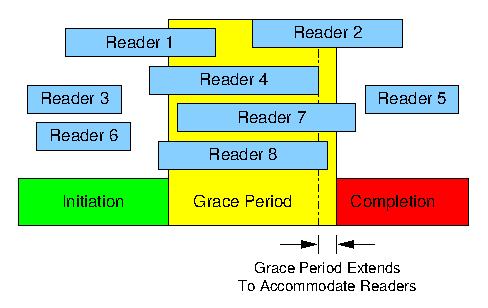
\includegraphics{advsync/RCUReaderGPExtends}}
\end{center}
\caption{RCU Readers Extending Grace Period}
\label{fig:advsync:RCU Readers Extending Grace Periods}
\end{figure}

The next sections show how these concepts can be applied to linked-list
data structures.

\subsection{Deletion From an RCU-Protected Linked List}
\label{sec:advsync:Deletion From an RCU-Protected Linked List}

Figure~\ref{fig:advsync:RCU Deletion From Linked List}
illustrates deletion from an RCU-protected linked list,
with time advancing from top to bottom.

\begin{figure}[htb]
\begin{center}
\resizebox{3in}{!}{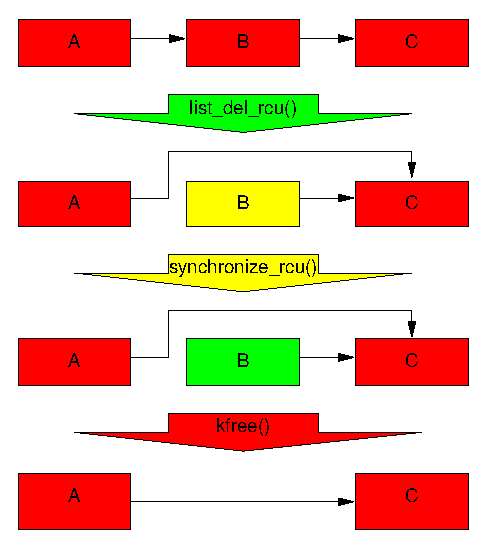
\includegraphics{advsync/RCUDeletion}}
\end{center}
\caption{RCU Deletion From Linked List}
\label{fig:advsync:RCU Deletion From Linked List}
\end{figure}

Initially, the list contains elements~A, B, and C, in that order.
RCU readers traverse the list concurrently with the update,
perhaps executing code like the following:

\vspace{5pt}
\begin{minipage}[t]{\columnwidth}
\begin{verbatim}
rcu_read_lock();
list_for_each_entry_rcu(p, h, le)
  if (p->key == k)
  	break;
present = p != NULL;
rcu_read_unlock();
\end{verbatim}
\end{minipage}
\vspace{5pt}

The \url{rcu_read_lock()} and \url{rcu_read_unlock()} primitives
delimit the RCU read-side critical section, preventing a grace
period from elapsing during this section of code.
Note that a grace period that commenced prior to the \url{rcu_read_lock()}
might complete during this critical section, but that a grace period
that begins after the \url{rcu_read_lock()} must not complete until
after completion of the \url{rcu_read_unlock()}.

Updaters might be executing code like the following:

\vspace{5pt}
\begin{minipage}[t]{\columnwidth}
\begin{verbatim}
/* p == element to delete. */
down(&update_sema);
list_del_rcu(p);
up(&update_sema);
synchronize_rcu();
kfree(p);
\end{verbatim}
\end{minipage}
\vspace{5pt}

The \url{down()} and \url{up()} Linux-kernel primitives act as sleeplock,
with \url{down()} acquiring the sleeplock ``\url{update_sema}''
and \url{up()} releasing it.

Note that both the \url{rcu_read_lock()} and \url{rcu_read_unlock()}
primitives have $O(1)$ execution time, and in particular, that
neither of them block or spin.
This means that the update code has no way of excluding readers.

Let us now walk through the execution of the update code
while referring to
Figure~\ref{fig:advsync:RCU Deletion From Linked List}.
A \url{list_del_rcu()} removes element~B from the list, so that
pre-existing readers might still be referencing
element~B, but new readers will advance from A directly to C.
Element~B's pointers remain intact, but so that readers still
referencing element~B will still advance to element~C.
A \url{synchronize_kernel()} waits for a grace period to elapse,
so that all readers that might have been referencing element~B have
advanced through the list.
Because new readers can no longer gain a reference to element~B,
it is now safe to execute \url{kfree()} to free up element~B's memory.

The \url{synchronize_rcu()} primitive can be thought of as a temporal
mutual-exclusion primitive, since it prevents the following \url{kfree()}
from executing until after any pre-existing readers complete.
The \url{kfree()} might well run concurrently with \emph{new}
RCU read-side critical sections, but it is guaranteed not to run
until after all \emph{old} RCU read-side critical sections complete.

The next section describes in-place update of an RCU-protected
linked list, the procedure that gave RCU its name.

\subsection{Replacement in an RCU-Protected Linked List}
\label{sec:advsync:Replacement in an RCU-Protected Linked List}

Figure~\ref{fig:advsync:RCU Replacement in Linked List}
shows how an RCU-protected data structure may be updated via
copying.
The read-side code is the same as for the previous exemple, but
the update code is outlined as follows:

\vspace{5pt}
\begin{minipage}[t]{\columnwidth}
\begin{verbatim}
down(&update_sema);
/* p == element to update */
q = kmalloc(sizeof(*q), GFP_KERNEL);
*q = *p;
list_replace_rcu(p, q);
up(&update_sema);
synchronize_rcu();
kfree(p);
\end{verbatim}
\end{minipage}
\vspace{5pt}

As before, we start with a linked list with elements~A, B, and C
in that order, and, again as before, readers might be traversing
this list throughout the update process.
To update element~B, we first allocate a new element and copy element~B
to it, then update the copy to produce element~B'.
We then execute \url{list_replace_rcu()} so that element~A now
references the new element~B' --- however, element~B still references
element~C so that any pre-existing readers still referencing old element~B
are still able to advance to element~C.
New readers will find element~B'.

After executing \url{synchronize_rcu()}, which again waits for a grace
period to elapse, all readers that were referencing old element~B'
will have advanced through the list, so that \url{kfree()} may now
be invoked on element~B, resulting in the final state with the list
now containing elements~A, B', and C.

This procedure where \emph{readers} continue traversing the list
while a \emph{copy} operation is used to carry out an \emph{update}
is what gives RCU --- or read-copy update --- its name.

\begin{figure}[p]
\begin{center}
\resizebox{3in}{!}{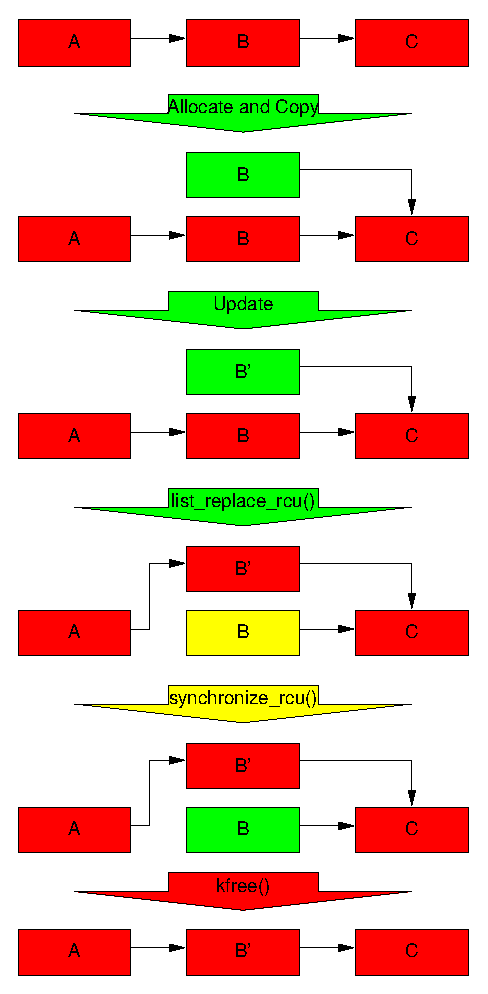
\includegraphics{advsync/RCUReplacement}}
\end{center}
\caption{RCU Replacement in Linked List}
\label{fig:advsync:RCU Replacement in Linked List}
\end{figure}

\subsection{Insertion into an RCU-Protected Linked List}
\label{sec:advsync:Insertion into an RCU-Protected Linked List}

Insertion into an RCU-protected linked list is straightforward, as
illustrated by
Figure~\ref{fig:advsync:RCU Insertion into Linked List}.
The read-side code is again that shown in
Section~\ref{sec:advsync:Deletion From an RCU-Protected Linked List},
and the update code might be as follows, where ``h'' is the list header:

\vspace{5pt}
\begin{minipage}[t]{\columnwidth}
\begin{verbatim}
down(&update_sema);
p = kmalloc(sizeof(*p), GFP_KERNEL);
initialize(p);
list_add_rcu(p, h);
up(&update_sema);
\end{verbatim}
\end{minipage}
\vspace{5pt}

Referring to
Figure~\ref{fig:advsync:RCU Insertion into Linked List},
the \url{kmalloc()} primitive and the programmer-supplied \url{initialize()}
function allocate and initialize the new element~B,
and the \url{list_add_rcu()} primitive inserts it into the list.
There is no need for grace periods in this case: readers will either
see the new element~B or not, depending on when they execute relative
to the update.

\begin{figure}[htb]
\begin{center}
\resizebox{3in}{!}{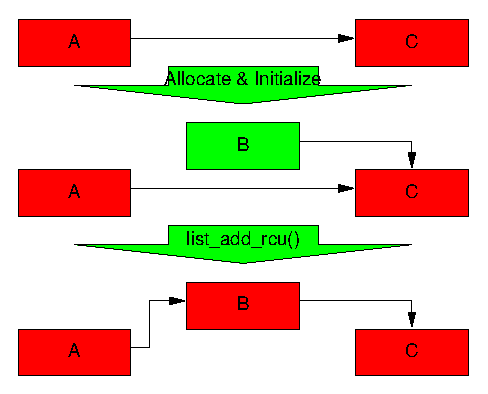
\includegraphics{advsync/RCUInsertion}}
\end{center}
\caption{RCU Insertion into Linked List}
\label{fig:advsync:RCU Insertion into Linked List}
\end{figure}

\subsection{RCU API}
\label{sec:advsync:RCU API}

RCU can be best thought of as an API, particularly given the large number
of implementations available for the RCU API.
Figure~\ref{fig:advsync:RCU API}
shows a color-coded guide to the major members of the Linux-kernel
RCU API, with the read-side primitives in blue boxes, the update-initiation
primitives in the green box, the grace-period primitives in the yellow box,
and the update-completion primitives in the red box.

\begin{figure}[htb]
\begin{center}
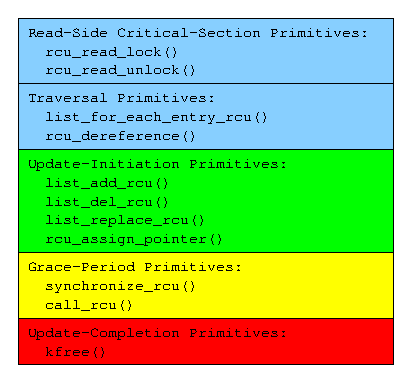
\includegraphics{advsync/RCU-API}
\end{center}
\caption{RCU API}
\label{fig:advsync:RCU API}
\end{figure}

As noted earlier, \url{rcu_read_lock()} and \url{rcu_read_unlock()}
delimit RCU read-side critical sections.
The \url{list_for_each_entry_rcu(p,h,f)} primitive is an iterator that
traverses the RCU-protected linked list with header ``h'' threaded
through struct field ``f'' using
local variable ``p'' as the iteration pointer.
The \url{rcu_dereference()} primitive is used to traverse RCU-protected
pointers, as in \url{rcu_dereference(p)->next}.

The \url{list_add_rcu()}, \url{list_del_rcu()}, and
\url{list_replace_rcu()} primitives perform the expected linked-list
operations, as illustrated in the examples in the preceding sections.
The \url{rcu_assign_pointer()} primitive assigns a new value to an
RCU-protected field, for example, \url{rcu_assign_pointer(p->next,q)}
would add the structure referenced by ``q'' following that referenced
by ``p''.

The \url{synchronize_rcu()} primitive waits for an RCU grace period
to elapse, as see in the examples in the previous sections.
The \url{call_rcu()} primitive causes a function to be invoked
at the end of a subsequent grace period, so that \url{call_rcu(p,f)}
would cause \url{f(p)} to be invoked after a grace period.
The \url{call_rcu()} primitive is thus the continuation form of the
\url{synchronize_rcu()} primitive.

Finally note that \url{kfree()} is simply an example, as any primitive
that frees memory can be used to complete an update.

The RCU API in the Linux kernel is somewhat more elaborate in order to
allow for the kernel's variety of different contexts and environments,
including interrupt and NMI handlers.

\QuickQuiz{Why is an {\tt rcu\_dereference()} primitive required?}{
	The {\tt rcu\_dereference()} primitive provides the memory
	barrier required by the DEC Alpha.
	Without such a memory barrier, the Alpha can dereference
	the new pointer and find pre-initialization data~\cite{Compaq01}.
	Perhaps more importantly, it serves to document which
	pointers are are protected by RCU.
	But most important of all, it disables compiler optimizations
	that might otherwise result in double fetches of the
	argument to {\tt rcu\_dereference()}.}
\QuickQuizEnd

\QuickQuiz{Why is a separate {\tt list\_for\_each\_entry\_rcu()} required?
	   In other words, why can't the existing
	   {\tt list\_for\_each\_entry()} primitive be used instead?}{
	The {\tt list\_for\_each\_entry\_rcu()} primitive includes the
	use of {\tt rcu\_dereference()} required by the DEC Alpha.}
\QuickQuizEnd

\QuickQuiz{Why would one need to use {\tt rcu\_assign\_pointer(p->next,q)} 
	   instead of the straightforward {\tt p->next=q}?}{
	On weakly consistent machines, a memory barrier is required
	between the initialization of a data structure and the
	assignment of the corresponding pointer that allows other
	CPUs to access the data structure.
	Without such a memory barrier, these other CPUs might
	see the assignments out of order, thus seeing the preinitialization
	contents of the data structure.
	The {\tt rcu\_assign\_pointer()} primitive includes such a
	memory barrier on any architectures requiring it.}
\QuickQuizEnd

\QuickQuiz{Why are there separate {\tt list\_add\_rcu()},
	   {\tt list\_del\_rcu()},
	   and {\tt list\_replace\_rcu()} primitives?
	   Why couldn't the existing {\tt list\_add()}, {\tt list\_del()},
	   and {\tt list\_replace()} primitives be used instead?}{
	The {\tt list\_add\_rcu()} and {\tt list\_replace\_rcu()} primitives
	must use the {\tt rcu\_assign\_pointer()} primitive
	(or, alternatively, explicit memory barriers).
	The {\tt list\_del\_rcu()} primitive must omit the ``poisoning''
	of list pointers that is used by {\tt list\_del()} as a
	debug check.}
\QuickQuizEnd

\subsection{RCU Properties}
\label{sec:advsync:RCU Properties}

The following are important properties of RCU, some of which are
beneficial, some adverse, and others dependent on the situation.

\begin{enumerate}
\item	Read-side primitives have very fast and deterministic
	execution time.
\item	Grace-period-detection primitives can have rather large
	and non-deterministic overheads.
\item	Read-side primitives cannot participate in a deadlock cycle.
\item	Read-side primitives cannot participate in a priority-inversion
	scenarios.
\item	When updates are guarded by locking, read-side critical
	sections can unconditionally acquire the update-side lock.
\item	Read-side critical sections run concurrently with updates.
	Without this read/update concurrency, the read-side primitives could
	not possibly be fast and deterministic, however, some algorithms
	do not straightforwardly tolerate such concurrency.
\item	Some implementations of the \url{call_rcu()} primitive
	can place very low overhead on the thread invoking
	\url{call_rcu()}, although the large overhead of grace-period
	detection is merely deferred, rather than avoided, in this
	case.
\end{enumerate}

RCU is therefore attractive in read-mostly situations where either
good performance and scalability or realtime response are required.
These properties will be discussed at greater length @@@.

@@@@ move RCU usage to its own chapter?

\begin{enumerate}
\item	Pure RCU~(\ref{sec:advsync:Pure RCU}).
\item	Reader-Writer-Lock/RCU
        Analogy~(\ref{sec:advsync:Reader-Writer-Lock/RCU Analogy}).
\item	RCU Existence Locks(\ref{sec:advsync:RCU Existence Locks}).
\item	RCU Readers With NBS
	Writers~(\ref{sec:advsync:RCU Readers With NBS Writers}).
\end{enumerate}

\subsection{Pure RCU}
\label{sec:advsync:Pure RCU}

Pure RCU is used to effect a lazy change in mode, for example, preventing
any new threads from accessing a subsystem, then waiting for all
pre-existing threads to complete before tearing it down.

\emph{@@@ Focus on change-in-mode uses.  (One can argue that the interrupt/NMI
uses are more closely related to reader-writer-lock/RCU analogy.)
Potential example: RCU guarding a variable prohibiting additional reference
counts for cleanup of the corresponding data structure.}

\subsection{Reader-Writer-Lock/RCU Analogy}
\label{sec:advsync:Reader-Writer-Lock/RCU Analogy}

\subsection{RCU Existence Locks}
\label{sec:advsync:RCU Existence Locks}

\subsection{RCU Readers With NBS Writers}
\label{sec:advsync:RCU Readers With NBS Writers}

\emph{@@@ simple intro, along with performance data on example from SMPdesign.}

\emph{@@@ consider moving advanced RCU usage to a separate chapter.
Add more material from chapter 5 of dissertation, particularly transformational
patterns.
\url{http://www.rdrop.com/users/paulmck/RCU/RCUdissertation.2004.07.14e1.pdf}.}

\emph{@@@ consider creating an RCU applications chapter/appendix, with
information from chapter 6 of dissertation.}
